\chapter{Methodology}
The main contributions of this thesis are new models of pose which allow us to 
incorporate new representations and features.  As such, in this part we show 
empirically that the methods are worthwhile by comparing them to 
state-of-the-art methods on competitive benchmark datasets.  Furthermore, we 
also analyze the trade-offs of the different models and the feature's 
effectiveness.

\section{Datasets}\label{sec:datasets}
\begin{figure}[tb]
\begin{center}
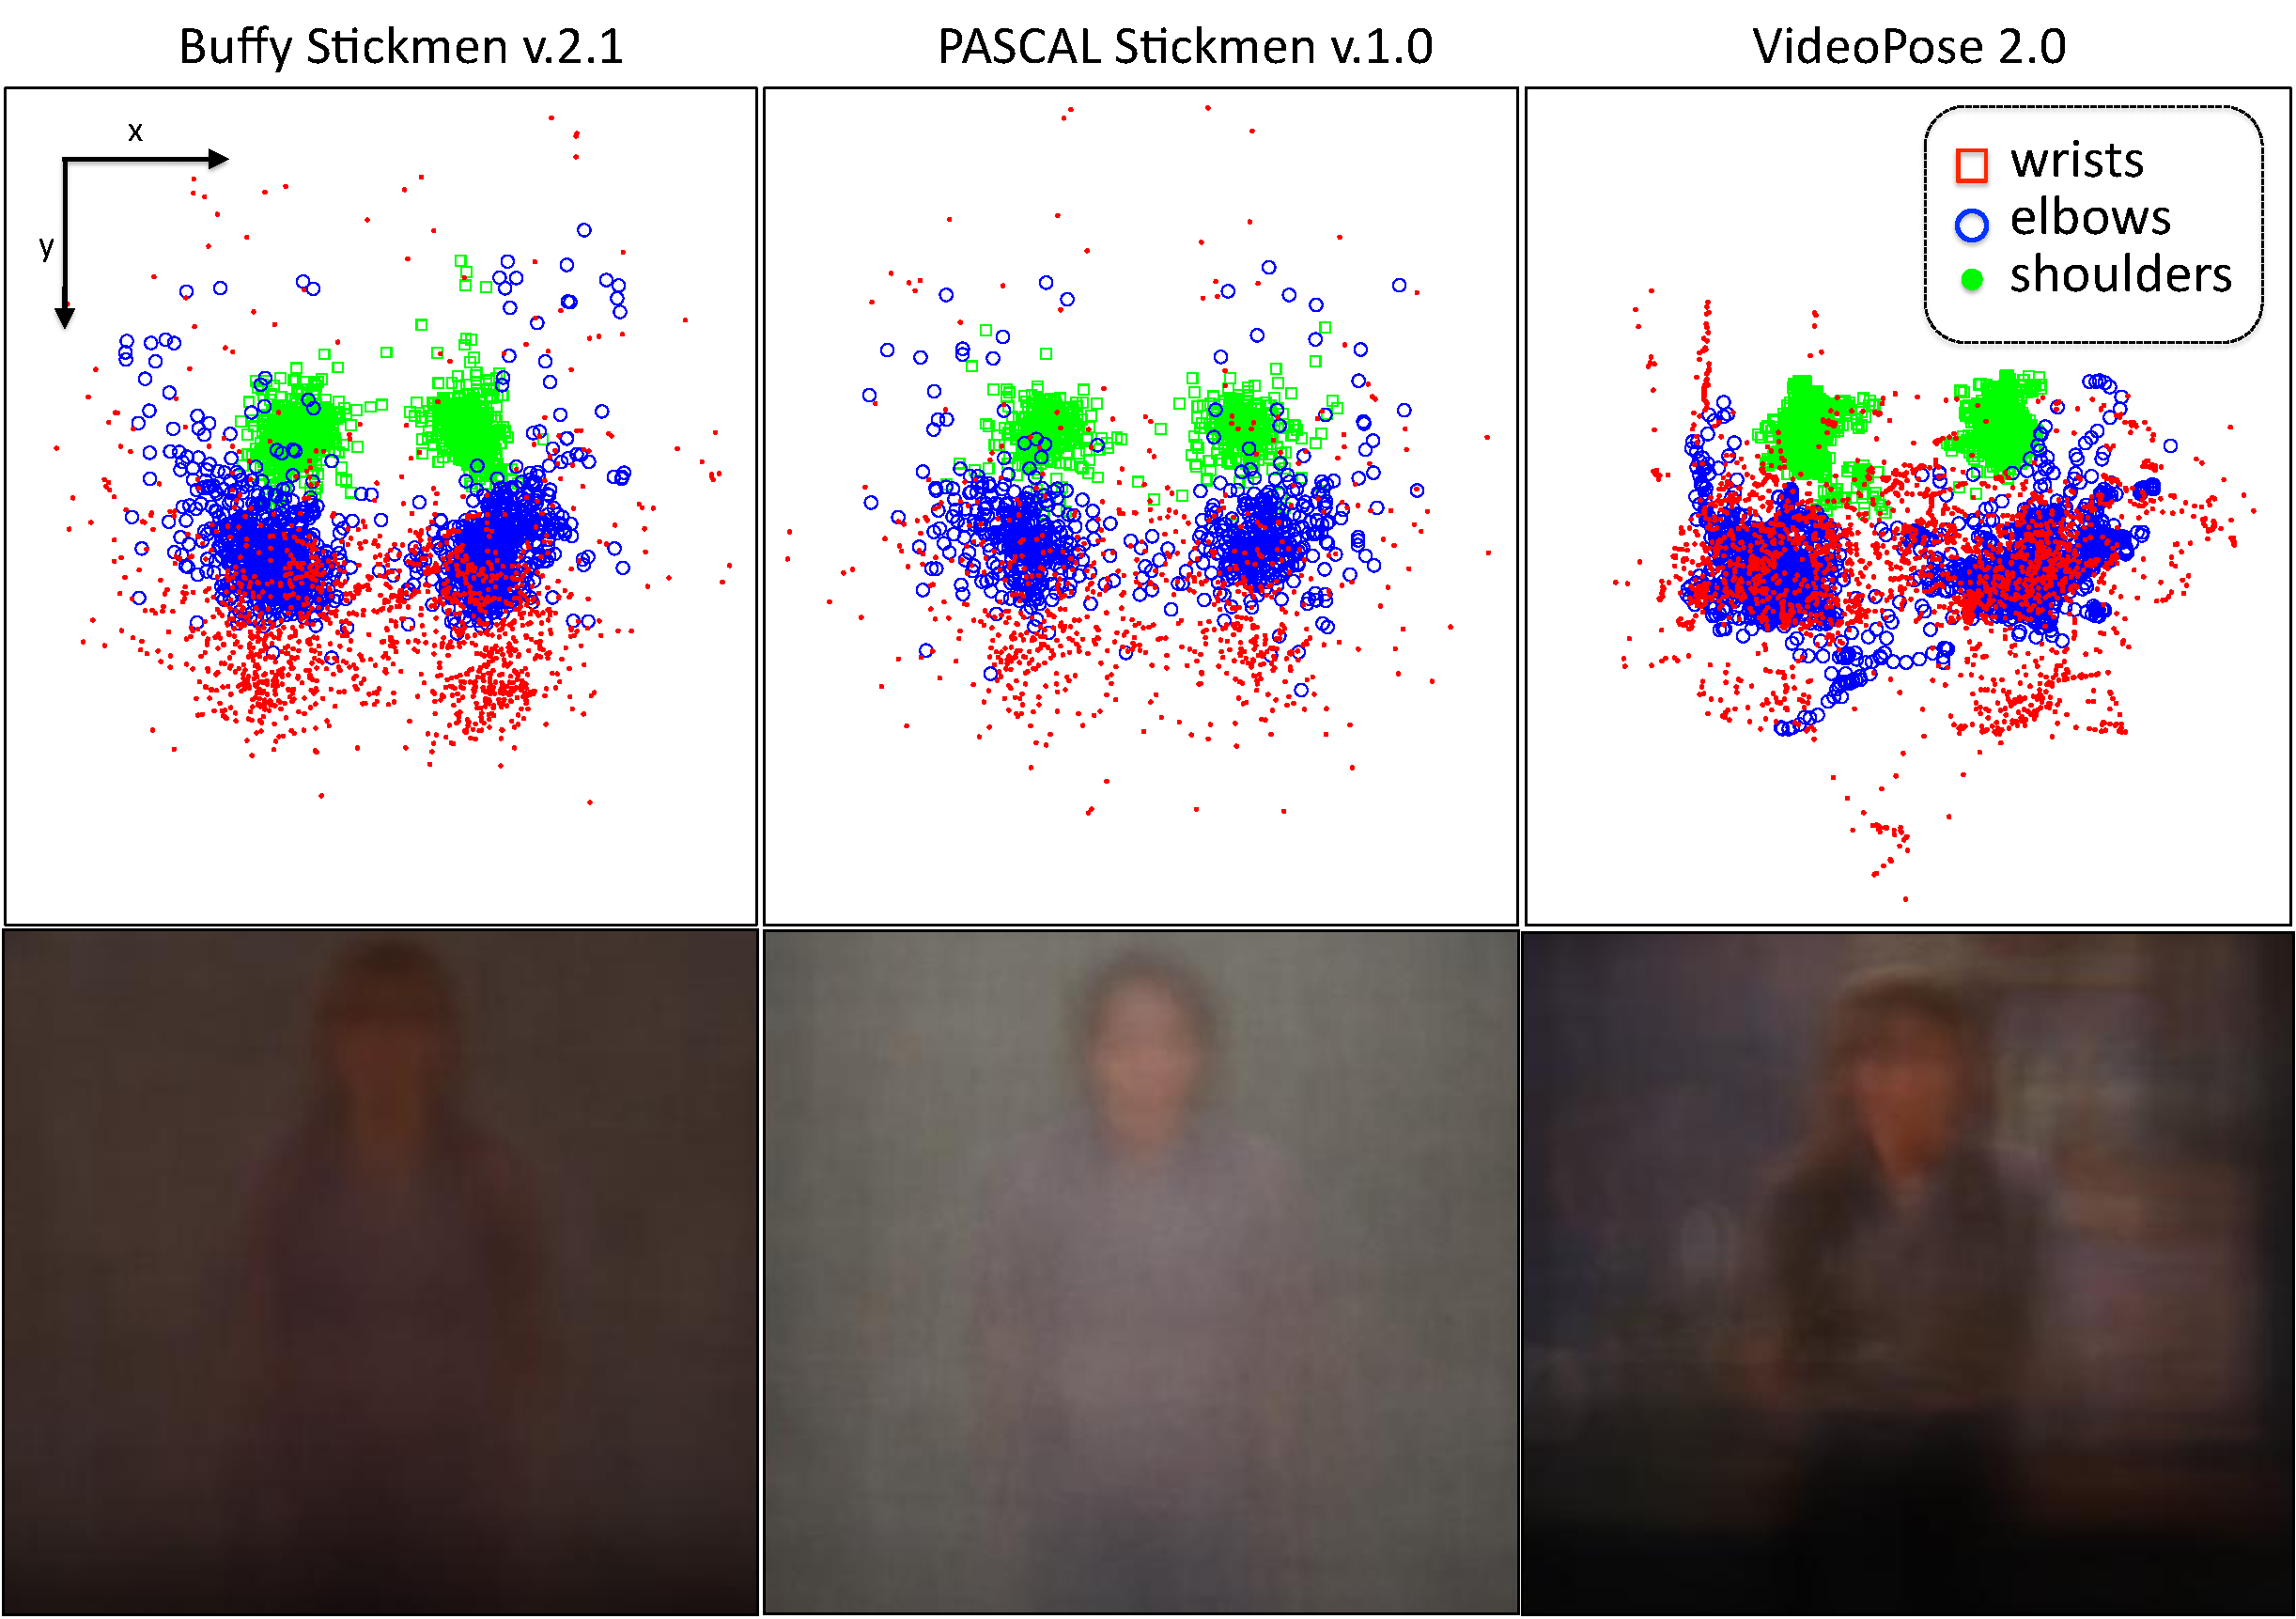
\includegraphics[width=1.05\textwidth]{figs/dataset-scatterplots.pdf}
\caption[Dataset joint scatterplots.]{Dataset joint scatterplots.  Here we show 
the spatial distribution of wrist, elbow and shoulder joints for our three 
datasets, both training and test.}
\label{fig:dataset-scatterplots}
\end{center}
\end{figure}



We evaluate our methods on three publicly available datasets

\subsection{Buffy Stickmen}
This dataset was first introduced in \citet{ferrari08}.  We use version 2.1 in 
our experiments, consisting of 748 frames from the TV show Buffy the Vampire 
Slayer, from episodes 2, 4, 5 and 6 from season 5.  The standard protocol is to 
test on a given set of 235 frames that were correctly localized by an upper 
body detector in~\citet{ferrari08}---within 50\% overlap with the groundtruth.  
For training images where an upper body detector did not detect a person for 
which we have annotated limbs, we loosely annotated the upper body manually to 
simulate test time behavior.
  

\subsection{PASCAL Stickmen}  This dataset was first introduced by 
\citet{eichner09} and contains 360 examples (version 1.0) obtained from amateur 
photographs culled from the PASCAL VOC 2008 challenge~\citep{voc09}.  This is 
purely a test dataset; the standard protocol is to train a model on Buffy 
images and test on PASCAL Stickmen. We follow this protocol for CPS, but for 
LLPS we have different needs, discussed in \secref{impl-details}.

\subsection{VideoPose}

We also apply our methods to a video dataset, which we collected ourselves: 
VideoPose 2.0.  Clips in the dataset were hand-selected (before developing our 
algorithm) to highlight natural settings where state-of-the-art methods fail: a 
highly varied (yet realistic) range of poses, rapid gesticulation, and a 
significant portion of frames (30\%) with foreshortened lower arms.  The 
dataset consists of 44 short clips, 2-3 seconds in length, with a total of 
1,286 frames.  We use 26 clips for training, recycle 1 training clip for a 
development set, and use 18 for testing.  As in the Buffy and PASCAL datasets, 
we fix global scale and translation of the person---in this case by manual 
annotation.


\subsection{Discussion} 


\section{Evaluation Measures}
\section{Competitor Methods}
\section{Implementation Details}


\chapter{Results}

\section{Feature analysis}


\section{System results}

